\documentclass[11pt]{article}
\usepackage[margin=1in]{geometry}
\usepackage{amsmath,amssymb,booktabs,graphicx,setspace,caption,hyperref}
\usepackage[T1]{fontenc}
\usepackage{mathpazo}
\setlength{\parindent}{0pt}
\setlength{\parskip}{0.6em}
\captionsetup{font=small,skip=6pt}
\title{Panel MS-AR(1): random intercepts with $E[z]=0$\\[0.4em]\large Seasonally adjusted real GDP per worker}
\author{}
\date{}
\begin{document}
\maketitle
\section{Model}
One specification. Joint panel Markov-switching AR(1) around a common linear trend, with Normal random intercepts. Outcome is log seasonally adjusted real GDP per worker (2026-09-17 vintage), full sample.
\begin{align}
y_{it} &= a_i + g\, t + z_{it}, \\
a_i &\sim \mathcal{N}(\alpha,\omega^2), \\
z_{i,t+1} &= \bigl(1-\rho(s_{it})\bigr)\mu(s_{it}) + \rho(s_{it})\, z_{it} + \sigma(s_{it})\,\varepsilon_{it}, \\
s_{i,t+1} &\sim \Pi(\,\cdot\mid s_{it}).
\end{align}
Three regimes. $\sigma$ and $\rho$ switch. $|\rho|<0.99$. The intercept and the regime means are not separately identified, so the unconditional mean of the cycle is restricted to $E[z]=0$ (the median regime mean is \emph{not} pinned at 0). Random intercepts use 11-point Gauss--Hermite. Plotted cycles use the posterior mean of $a_i$. Standard errors are delta-method from a numerical Hessian.
\clearpage
\section{Random intercepts, common linear trend, E[z]=0}
2026-09-17 SA panel, full sample, $y_{it}=a_i+gt+z_{it}$, $E[z]=0$. 74 countries, 8670 observations, 1950-Q1--2026-Q2. Fitted countries: 74. Observations: 8670. Log-likelihood: 23496.84.
Random intercepts $a_i\sim N(\alpha,\omega^2)$ with $\alpha=-5.1672$ (0.0529), $\omega=0.5041$ (0.0058). Posterior-mean $a_i$: mean -5.220, min -7.782, max -3.640. Common slope $g=0.0055$ (0.0007).
\begin{table}[h]
\centering
\caption{Regime AR(1), transition matrix, and ergodic $\pi$. Columns are regimes.}
\begin{tabular}{lccc}
\toprule
 & (0) & (1) & (2) \\
\midrule
$\mu$ & -1.0703 & -0.0794 & 0.2903 \\
 & (0.0963) & --- & (0.0233) \\ \addlinespace
$\sigma$ & 0.0738 & 0.0186 & 0.0069 \\
 & (0.0025) & (0.0005) & (0.0001) \\ \addlinespace
$\rho$ & 0.9899 & 0.9900 & 0.9899 \\
 & (0.0005) & (0.0001) & (0.0001) \\ \addlinespace
$\Pi_{0\cdot}$ & 0.6943 & 0.2876 & 0.0181 \\
 & (0.0323) & (0.0329) & (0.0083) \\ \addlinespace
$\Pi_{1\cdot}$ & 0.0638 & 0.8778 & 0.0584 \\
 & (0.0079) & (0.0109) & (0.0068) \\ \addlinespace
$\Pi_{2\cdot}$ & 0.0052 & 0.0506 & 0.9442 \\
 & (0.0033) & (0.0067) & (0.0055) \\ \addlinespace
$\pi$ & 0.0971 & 0.4262 & 0.4767 \\
 & (0.0100) & (0.0209) & (0.0248) \\ \addlinespace
\bottomrule
\end{tabular}
\end{table}
\begin{figure}[h]
\centering
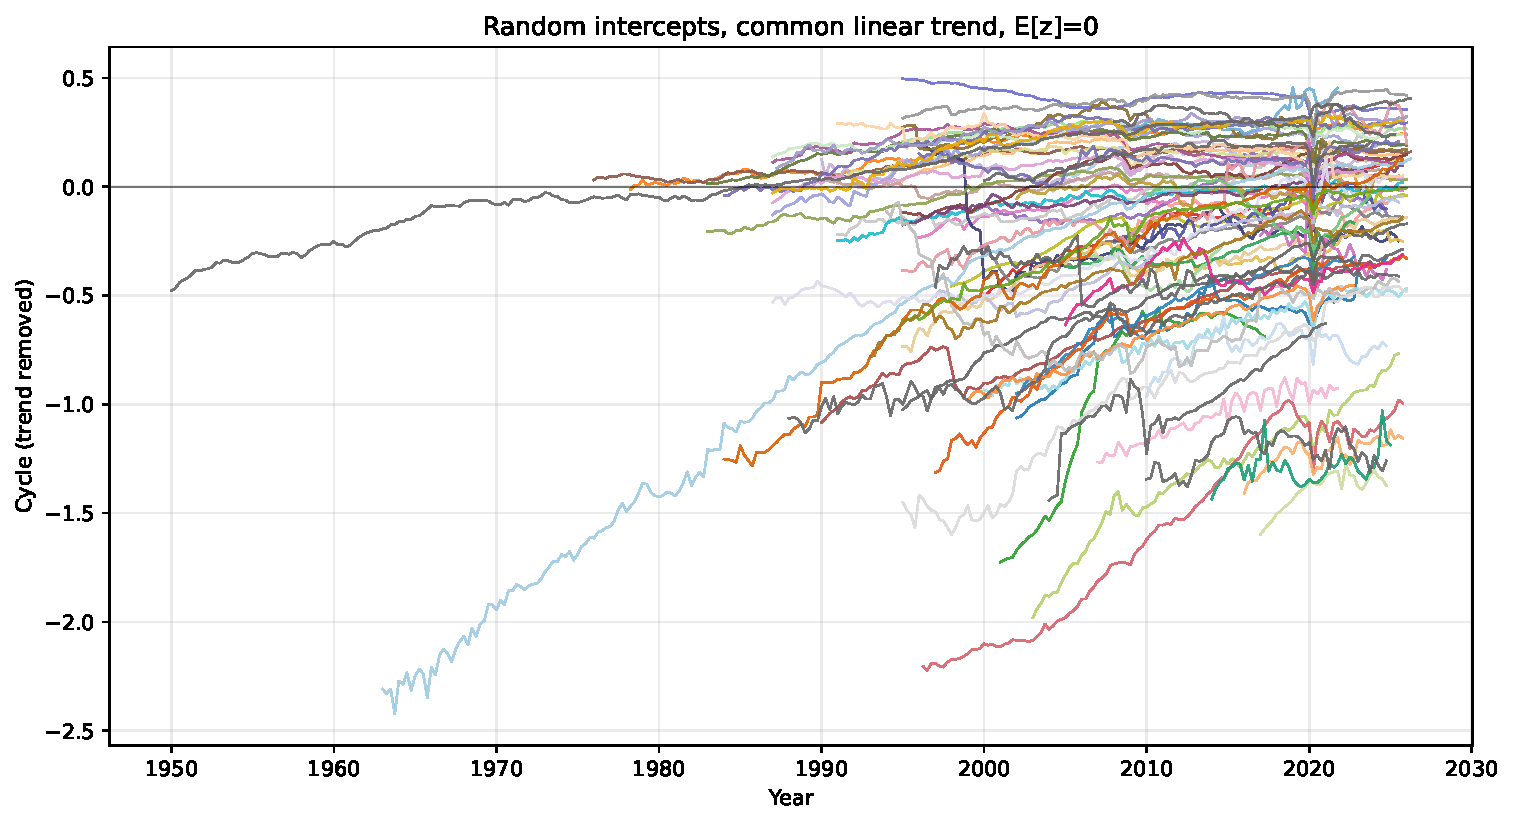
\includegraphics[width=0.75\textwidth]{figs/cycle_re_ez0.pdf}
\caption{Country cycles after removing the posterior-mean intercept and the common linear trend.}
\end{figure}
\end{document}
